\chapter{Planning and Conducting Empirical Studies}

\section{The PPDAC framework}

Stat 231 organizes every empirical study into five stages, abbreviated \textbf{PPDAC}:
\textbf{P}roblem, \textbf{P}lan, \textbf{D}ata, \textbf{A}nalysis, \textbf{C}onclusion.
The framework is a checklist for designing a study and for critically reading someone
else's.

\begin{center}
\begin{tikzpicture}[node distance=0.6cm, box/.style={draw, rounded corners, minimum width=2cm, minimum height=0.8cm, align=center}]
  \node[box] (p1) {Problem};
  \node[box, right=of p1] (p2) {Plan};
  \node[box, right=of p2] (d) {Data};
  \node[box, right=of d] (a) {Analysis};
  \node[box, right=of a] (c) {Conclusion};
  \draw[-{Stealth}] (p1) -- (p2);
  \draw[-{Stealth}] (p2) -- (d);
  \draw[-{Stealth}] (d) -- (a);
  \draw[-{Stealth}] (a) -- (c);
  \draw[-{Stealth}, dashed] (c.south) to[bend left=20] node[below] {\small new questions} (p1.south);
\end{tikzpicture}
\end{center}

\subsection{Problem}
A clear statement of what we want to learn.
\begin{itemize}
  \item \textbf{Target population/process}: the collection of units to which we want
        the conclusions to apply.
  \item \textbf{Variates}: response variate(s) $y$ and explanatory variate(s) $x$.
  \item \textbf{Attributes} of interest: e.g.\ the mean of $y$, a proportion, a
        difference of means between two groups.
  \item \textbf{Type of question}: descriptive, causative or predictive.
\end{itemize}

\subsection{Plan}
How the data will be collected.
\begin{itemize}
  \item \textbf{Study population}: the collection of units that \emph{could} be
        selected in the study. Often different from the target population (e.g.\ target:
        all Canadian adults; study population: adults with a listed phone number; or
        target: humans, study population: laboratory mice).
  \item \textbf{Sampling protocol}: how units are selected from the study population, and
        the sample size $n$.
  \item \textbf{Measurement system}: how the variates are measured (instruments,
        questionnaire wording, who measures, when).
  \item For experiments: how the explanatory variates are assigned to units.
\end{itemize}

\subsection{Data}
Collect the data according to the plan, recording any departures from it (non-response,
lost units, measurement problems). Data should be checked and cleaned and stored
in a format suitable for analysis.

\subsection{Analysis}
Numerical and graphical summaries (Chapter 1), choice and fitting of a model
(Chapter 2), estimation and testing (Chapters 4--7), and model checking.

\subsection{Conclusion}
Answer the question posed in the Problem step, in plain language, together with a
statement of uncertainty and a discussion of the limitations of the study, in particular
the errors described next.

\section{Errors in a study}

The difference between the conclusions of a study and the truth about the target
population comes from three sources.

\begin{definition}[Study, sample and measurement error]
\begin{itemize}
  \item \textbf{Study error}: the difference between the attribute in the
        \emph{study population} and the attribute in the \emph{target population}.
        It cannot be reduced by taking a bigger sample and cannot be quantified from the
        data; it must be argued from context.
  \item \textbf{Sample error}: the difference between the attribute in the
        \emph{sample} and the attribute in the \emph{study population}. With a random
        sampling protocol, sample error can be modelled with probability and quantified
        (confidence intervals); it decreases as $n$ grows.
  \item \textbf{Measurement error}: the difference between the measured value of a
        variate and its true value. It may be random (imprecision) or systematic
        (bias, e.g.\ a mis-calibrated scale, a leading survey question).
\end{itemize}
\end{definition}

\begin{center}
\begin{tikzpicture}[every node/.style={font=\small}]
  \draw[fill=blue!6] (0,0) ellipse (5.2 and 2.2);
  \draw[fill=blue!14] (1.0,-0.2) ellipse (3.0 and 1.5);
  \draw[fill=blue!30] (1.9,-0.4) ellipse (1.1 and 0.7);
  \node[align=center] at (-3.5,0.7) {target\\population};
  \node[align=center] at (-0.5,0.6) {study\\population};
  \node at (1.9,-0.4) {sample};
  \draw[{Stealth}-{Stealth}, red!70!black] (-5.08,-0.4) -- node[below, font=\scriptsize] {study error} (-1.97,-0.4);
  \draw[{Stealth}-{Stealth}, red!70!black] (-1.97,-0.4) -- node[below, font=\scriptsize] {sample error} (0.8,-0.4);
  \node[draw, rounded corners, fill=white, font=\scriptsize, align=center] (m) at (6.7,-0.4) {\textcolor{red!70!black}{measurement error:}\\measured vs.\ true value};
  \draw[-{Stealth}, red!70!black] (m) -- (3.0,-0.4);
\end{tikzpicture}
\end{center}
The three populations are nested: conclusions travel from the sample to the study
population (sample error) and then, by argument rather than by data, to the target
population (study error); every value recorded along the way carries measurement error.

\begin{example}[Identifying the errors]
A researcher wants the average weekly hours of exercise of Ontario university students.
She emails a survey to $5000$ students chosen at random from the UW registrar's list; $900$
reply. Students report their own exercise hours for ``a typical week''.
\begin{itemize}
  \item Target population: Ontario university students. Study population: UW students
        on the registrar's list. \emph{Study error}: UW students may exercise more or less
        than students elsewhere.
  \item Sample error: even a perfect random sample of $900$ UW students would not have
        exactly the UW mean. Worse, the $18\%$ who replied are self-selected
        (\emph{non-response bias}); keen exercisers may be more likely to answer.
  \item Measurement error: self-reported exercise is typically overstated (systematic)
        and ``typical week'' is vague (random).
\end{itemize}
\end{example}

\section{Sampling protocols}

\begin{definition}[Simple random sampling]
A \emph{simple random sample} (SRS) of size $n$ from a study population of $N$ units is
chosen so that every subset of $n$ units has the same probability $1/\binom Nn$ of being
selected. It requires a list of the population (a \emph{sampling frame}) and a random
number generator.
\end{definition}

Random sampling is what justifies the probability models of the later chapters: under
an SRS, the sample is ``representative on average'' and the sample error has a known
distribution. Other protocols:
\begin{itemize}
  \item \textbf{Stratified sampling}: divide the population into groups (strata, e.g.\
        faculties) and take an SRS within each. Ensures every stratum is represented and
        often improves precision.
  \item \textbf{Cluster sampling}: randomly select whole groups (e.g.\ classrooms) and
        measure all units in them. Cheaper, but usually less precise.
  \item \textbf{Systematic sampling}: every $k$th unit from a list after a random start.
  \item \textbf{Convenience / volunteer sampling}: whoever is easiest to reach or chooses
        to respond. Cheap but prone to serious, unquantifiable bias.
\end{itemize}

\begin{center}
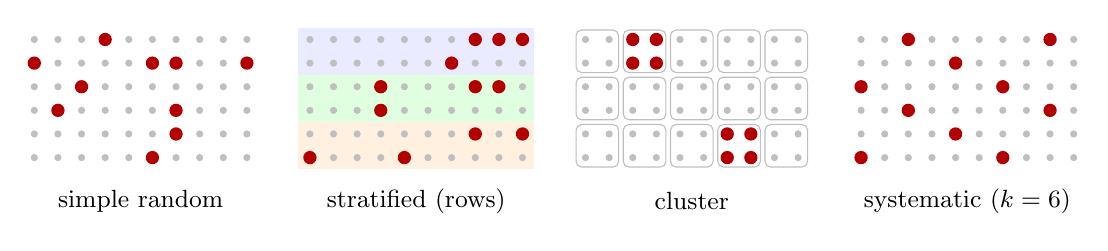
\begin{tikzpicture}
  \begin{scope}[xshift=0cm]
    \fill[gray!50] (0.00,0.00) circle (1.3pt);
    \fill[gray!50] (0.00,0.30) circle (1.3pt);
    \fill[gray!50] (0.00,0.60) circle (1.3pt);
    \fill[gray!50] (0.00,0.90) circle (1.3pt);
    \fill[red!70!black] (0.00,1.20) circle (2.4pt);
    \fill[gray!50] (0.00,1.50) circle (1.3pt);
    \fill[gray!50] (0.30,0.00) circle (1.3pt);
    \fill[gray!50] (0.30,0.30) circle (1.3pt);
    \fill[red!70!black] (0.30,0.60) circle (2.4pt);
    \fill[gray!50] (0.30,0.90) circle (1.3pt);
    \fill[gray!50] (0.30,1.20) circle (1.3pt);
    \fill[gray!50] (0.30,1.50) circle (1.3pt);
    \fill[gray!50] (0.60,0.00) circle (1.3pt);
    \fill[gray!50] (0.60,0.30) circle (1.3pt);
    \fill[gray!50] (0.60,0.60) circle (1.3pt);
    \fill[red!70!black] (0.60,0.90) circle (2.4pt);
    \fill[gray!50] (0.60,1.20) circle (1.3pt);
    \fill[gray!50] (0.60,1.50) circle (1.3pt);
    \fill[gray!50] (0.90,0.00) circle (1.3pt);
    \fill[gray!50] (0.90,0.30) circle (1.3pt);
    \fill[gray!50] (0.90,0.60) circle (1.3pt);
    \fill[gray!50] (0.90,0.90) circle (1.3pt);
    \fill[gray!50] (0.90,1.20) circle (1.3pt);
    \fill[red!70!black] (0.90,1.50) circle (2.4pt);
    \fill[gray!50] (1.20,0.00) circle (1.3pt);
    \fill[gray!50] (1.20,0.30) circle (1.3pt);
    \fill[gray!50] (1.20,0.60) circle (1.3pt);
    \fill[gray!50] (1.20,0.90) circle (1.3pt);
    \fill[gray!50] (1.20,1.20) circle (1.3pt);
    \fill[gray!50] (1.20,1.50) circle (1.3pt);
    \fill[red!70!black] (1.50,0.00) circle (2.4pt);
    \fill[gray!50] (1.50,0.30) circle (1.3pt);
    \fill[gray!50] (1.50,0.60) circle (1.3pt);
    \fill[gray!50] (1.50,0.90) circle (1.3pt);
    \fill[red!70!black] (1.50,1.20) circle (2.4pt);
    \fill[gray!50] (1.50,1.50) circle (1.3pt);
    \fill[gray!50] (1.80,0.00) circle (1.3pt);
    \fill[red!70!black] (1.80,0.30) circle (2.4pt);
    \fill[red!70!black] (1.80,0.60) circle (2.4pt);
    \fill[gray!50] (1.80,0.90) circle (1.3pt);
    \fill[red!70!black] (1.80,1.20) circle (2.4pt);
    \fill[gray!50] (1.80,1.50) circle (1.3pt);
    \fill[gray!50] (2.10,0.00) circle (1.3pt);
    \fill[gray!50] (2.10,0.30) circle (1.3pt);
    \fill[gray!50] (2.10,0.60) circle (1.3pt);
    \fill[gray!50] (2.10,0.90) circle (1.3pt);
    \fill[gray!50] (2.10,1.20) circle (1.3pt);
    \fill[gray!50] (2.10,1.50) circle (1.3pt);
    \fill[gray!50] (2.40,0.00) circle (1.3pt);
    \fill[gray!50] (2.40,0.30) circle (1.3pt);
    \fill[gray!50] (2.40,0.60) circle (1.3pt);
    \fill[gray!50] (2.40,0.90) circle (1.3pt);
    \fill[gray!50] (2.40,1.20) circle (1.3pt);
    \fill[gray!50] (2.40,1.50) circle (1.3pt);
    \fill[gray!50] (2.70,0.00) circle (1.3pt);
    \fill[gray!50] (2.70,0.30) circle (1.3pt);
    \fill[gray!50] (2.70,0.60) circle (1.3pt);
    \fill[gray!50] (2.70,0.90) circle (1.3pt);
    \fill[red!70!black] (2.70,1.20) circle (2.4pt);
    \fill[gray!50] (2.70,1.50) circle (1.3pt);
    \node[font=\small] at (1.35,-0.55) {simple random};
  \end{scope}
  \begin{scope}[xshift=3.5cm]
    \fill[orange!12] (-0.15,-0.15) rectangle (2.85,0.44999999999999996);
    \fill[green!12] (-0.15,0.44999999999999996) rectangle (2.85,1.05);
    \fill[blue!8] (-0.15,1.05) rectangle (2.85,1.65);
    \fill[red!70!black] (0.00,0.00) circle (2.4pt);
    \fill[gray!50] (0.00,0.30) circle (1.3pt);
    \fill[gray!50] (0.00,0.60) circle (1.3pt);
    \fill[gray!50] (0.00,0.90) circle (1.3pt);
    \fill[gray!50] (0.00,1.20) circle (1.3pt);
    \fill[gray!50] (0.00,1.50) circle (1.3pt);
    \fill[gray!50] (0.30,0.00) circle (1.3pt);
    \fill[gray!50] (0.30,0.30) circle (1.3pt);
    \fill[gray!50] (0.30,0.60) circle (1.3pt);
    \fill[gray!50] (0.30,0.90) circle (1.3pt);
    \fill[gray!50] (0.30,1.20) circle (1.3pt);
    \fill[gray!50] (0.30,1.50) circle (1.3pt);
    \fill[gray!50] (0.60,0.00) circle (1.3pt);
    \fill[gray!50] (0.60,0.30) circle (1.3pt);
    \fill[gray!50] (0.60,0.60) circle (1.3pt);
    \fill[gray!50] (0.60,0.90) circle (1.3pt);
    \fill[gray!50] (0.60,1.20) circle (1.3pt);
    \fill[gray!50] (0.60,1.50) circle (1.3pt);
    \fill[gray!50] (0.90,0.00) circle (1.3pt);
    \fill[gray!50] (0.90,0.30) circle (1.3pt);
    \fill[red!70!black] (0.90,0.60) circle (2.4pt);
    \fill[red!70!black] (0.90,0.90) circle (2.4pt);
    \fill[gray!50] (0.90,1.20) circle (1.3pt);
    \fill[gray!50] (0.90,1.50) circle (1.3pt);
    \fill[red!70!black] (1.20,0.00) circle (2.4pt);
    \fill[gray!50] (1.20,0.30) circle (1.3pt);
    \fill[gray!50] (1.20,0.60) circle (1.3pt);
    \fill[gray!50] (1.20,0.90) circle (1.3pt);
    \fill[gray!50] (1.20,1.20) circle (1.3pt);
    \fill[gray!50] (1.20,1.50) circle (1.3pt);
    \fill[gray!50] (1.50,0.00) circle (1.3pt);
    \fill[gray!50] (1.50,0.30) circle (1.3pt);
    \fill[gray!50] (1.50,0.60) circle (1.3pt);
    \fill[gray!50] (1.50,0.90) circle (1.3pt);
    \fill[gray!50] (1.50,1.20) circle (1.3pt);
    \fill[gray!50] (1.50,1.50) circle (1.3pt);
    \fill[gray!50] (1.80,0.00) circle (1.3pt);
    \fill[gray!50] (1.80,0.30) circle (1.3pt);
    \fill[gray!50] (1.80,0.60) circle (1.3pt);
    \fill[gray!50] (1.80,0.90) circle (1.3pt);
    \fill[red!70!black] (1.80,1.20) circle (2.4pt);
    \fill[gray!50] (1.80,1.50) circle (1.3pt);
    \fill[gray!50] (2.10,0.00) circle (1.3pt);
    \fill[red!70!black] (2.10,0.30) circle (2.4pt);
    \fill[gray!50] (2.10,0.60) circle (1.3pt);
    \fill[red!70!black] (2.10,0.90) circle (2.4pt);
    \fill[gray!50] (2.10,1.20) circle (1.3pt);
    \fill[red!70!black] (2.10,1.50) circle (2.4pt);
    \fill[gray!50] (2.40,0.00) circle (1.3pt);
    \fill[gray!50] (2.40,0.30) circle (1.3pt);
    \fill[gray!50] (2.40,0.60) circle (1.3pt);
    \fill[red!70!black] (2.40,0.90) circle (2.4pt);
    \fill[gray!50] (2.40,1.20) circle (1.3pt);
    \fill[red!70!black] (2.40,1.50) circle (2.4pt);
    \fill[gray!50] (2.70,0.00) circle (1.3pt);
    \fill[red!70!black] (2.70,0.30) circle (2.4pt);
    \fill[gray!50] (2.70,0.60) circle (1.3pt);
    \fill[gray!50] (2.70,0.90) circle (1.3pt);
    \fill[gray!50] (2.70,1.20) circle (1.3pt);
    \fill[red!70!black] (2.70,1.50) circle (2.4pt);
    \node[font=\small] at (1.35,-0.55) {stratified (rows)};
  \end{scope}
  \begin{scope}[xshift=7cm]
    \draw[gray!50, rounded corners=2pt] (-0.12,-0.12) rectangle (0.42,0.42);
    \draw[gray!50, rounded corners=2pt] (-0.12,0.48) rectangle (0.42,1.02);
    \draw[gray!50, rounded corners=2pt] (-0.12,1.08) rectangle (0.42,1.6199999999999999);
    \draw[gray!50, rounded corners=2pt] (0.48,-0.12) rectangle (1.02,0.42);
    \draw[gray!50, rounded corners=2pt] (0.48,0.48) rectangle (1.02,1.02);
    \draw[gray!50, rounded corners=2pt] (0.48,1.08) rectangle (1.02,1.6199999999999999);
    \draw[gray!50, rounded corners=2pt] (1.08,-0.12) rectangle (1.6199999999999999,0.42);
    \draw[gray!50, rounded corners=2pt] (1.08,0.48) rectangle (1.6199999999999999,1.02);
    \draw[gray!50, rounded corners=2pt] (1.08,1.08) rectangle (1.6199999999999999,1.6199999999999999);
    \draw[gray!50, rounded corners=2pt] (1.6799999999999997,-0.12) rectangle (2.2199999999999998,0.42);
    \draw[gray!50, rounded corners=2pt] (1.6799999999999997,0.48) rectangle (2.2199999999999998,1.02);
    \draw[gray!50, rounded corners=2pt] (1.6799999999999997,1.08) rectangle (2.2199999999999998,1.6199999999999999);
    \draw[gray!50, rounded corners=2pt] (2.28,-0.12) rectangle (2.82,0.42);
    \draw[gray!50, rounded corners=2pt] (2.28,0.48) rectangle (2.82,1.02);
    \draw[gray!50, rounded corners=2pt] (2.28,1.08) rectangle (2.82,1.6199999999999999);
    \fill[gray!50] (0.00,0.00) circle (1.3pt);
    \fill[gray!50] (0.00,0.30) circle (1.3pt);
    \fill[gray!50] (0.00,0.60) circle (1.3pt);
    \fill[gray!50] (0.00,0.90) circle (1.3pt);
    \fill[gray!50] (0.00,1.20) circle (1.3pt);
    \fill[gray!50] (0.00,1.50) circle (1.3pt);
    \fill[gray!50] (0.30,0.00) circle (1.3pt);
    \fill[gray!50] (0.30,0.30) circle (1.3pt);
    \fill[gray!50] (0.30,0.60) circle (1.3pt);
    \fill[gray!50] (0.30,0.90) circle (1.3pt);
    \fill[gray!50] (0.30,1.20) circle (1.3pt);
    \fill[gray!50] (0.30,1.50) circle (1.3pt);
    \fill[gray!50] (0.60,0.00) circle (1.3pt);
    \fill[gray!50] (0.60,0.30) circle (1.3pt);
    \fill[gray!50] (0.60,0.60) circle (1.3pt);
    \fill[gray!50] (0.60,0.90) circle (1.3pt);
    \fill[red!70!black] (0.60,1.20) circle (2.4pt);
    \fill[red!70!black] (0.60,1.50) circle (2.4pt);
    \fill[gray!50] (0.90,0.00) circle (1.3pt);
    \fill[gray!50] (0.90,0.30) circle (1.3pt);
    \fill[gray!50] (0.90,0.60) circle (1.3pt);
    \fill[gray!50] (0.90,0.90) circle (1.3pt);
    \fill[red!70!black] (0.90,1.20) circle (2.4pt);
    \fill[red!70!black] (0.90,1.50) circle (2.4pt);
    \fill[gray!50] (1.20,0.00) circle (1.3pt);
    \fill[gray!50] (1.20,0.30) circle (1.3pt);
    \fill[gray!50] (1.20,0.60) circle (1.3pt);
    \fill[gray!50] (1.20,0.90) circle (1.3pt);
    \fill[gray!50] (1.20,1.20) circle (1.3pt);
    \fill[gray!50] (1.20,1.50) circle (1.3pt);
    \fill[gray!50] (1.50,0.00) circle (1.3pt);
    \fill[gray!50] (1.50,0.30) circle (1.3pt);
    \fill[gray!50] (1.50,0.60) circle (1.3pt);
    \fill[gray!50] (1.50,0.90) circle (1.3pt);
    \fill[gray!50] (1.50,1.20) circle (1.3pt);
    \fill[gray!50] (1.50,1.50) circle (1.3pt);
    \fill[red!70!black] (1.80,0.00) circle (2.4pt);
    \fill[red!70!black] (1.80,0.30) circle (2.4pt);
    \fill[gray!50] (1.80,0.60) circle (1.3pt);
    \fill[gray!50] (1.80,0.90) circle (1.3pt);
    \fill[gray!50] (1.80,1.20) circle (1.3pt);
    \fill[gray!50] (1.80,1.50) circle (1.3pt);
    \fill[red!70!black] (2.10,0.00) circle (2.4pt);
    \fill[red!70!black] (2.10,0.30) circle (2.4pt);
    \fill[gray!50] (2.10,0.60) circle (1.3pt);
    \fill[gray!50] (2.10,0.90) circle (1.3pt);
    \fill[gray!50] (2.10,1.20) circle (1.3pt);
    \fill[gray!50] (2.10,1.50) circle (1.3pt);
    \fill[gray!50] (2.40,0.00) circle (1.3pt);
    \fill[gray!50] (2.40,0.30) circle (1.3pt);
    \fill[gray!50] (2.40,0.60) circle (1.3pt);
    \fill[gray!50] (2.40,0.90) circle (1.3pt);
    \fill[gray!50] (2.40,1.20) circle (1.3pt);
    \fill[gray!50] (2.40,1.50) circle (1.3pt);
    \fill[gray!50] (2.70,0.00) circle (1.3pt);
    \fill[gray!50] (2.70,0.30) circle (1.3pt);
    \fill[gray!50] (2.70,0.60) circle (1.3pt);
    \fill[gray!50] (2.70,0.90) circle (1.3pt);
    \fill[gray!50] (2.70,1.20) circle (1.3pt);
    \fill[gray!50] (2.70,1.50) circle (1.3pt);
    \node[font=\small] at (1.35,-0.55) {cluster};
  \end{scope}
  \begin{scope}[xshift=10.5cm]
    \fill[red!70!black] (0.00,0.00) circle (2.4pt);
    \fill[gray!50] (0.00,0.30) circle (1.3pt);
    \fill[gray!50] (0.00,0.60) circle (1.3pt);
    \fill[red!70!black] (0.00,0.90) circle (2.4pt);
    \fill[gray!50] (0.00,1.20) circle (1.3pt);
    \fill[gray!50] (0.00,1.50) circle (1.3pt);
    \fill[gray!50] (0.30,0.00) circle (1.3pt);
    \fill[gray!50] (0.30,0.30) circle (1.3pt);
    \fill[gray!50] (0.30,0.60) circle (1.3pt);
    \fill[gray!50] (0.30,0.90) circle (1.3pt);
    \fill[gray!50] (0.30,1.20) circle (1.3pt);
    \fill[gray!50] (0.30,1.50) circle (1.3pt);
    \fill[gray!50] (0.60,0.00) circle (1.3pt);
    \fill[gray!50] (0.60,0.30) circle (1.3pt);
    \fill[red!70!black] (0.60,0.60) circle (2.4pt);
    \fill[gray!50] (0.60,0.90) circle (1.3pt);
    \fill[gray!50] (0.60,1.20) circle (1.3pt);
    \fill[red!70!black] (0.60,1.50) circle (2.4pt);
    \fill[gray!50] (0.90,0.00) circle (1.3pt);
    \fill[gray!50] (0.90,0.30) circle (1.3pt);
    \fill[gray!50] (0.90,0.60) circle (1.3pt);
    \fill[gray!50] (0.90,0.90) circle (1.3pt);
    \fill[gray!50] (0.90,1.20) circle (1.3pt);
    \fill[gray!50] (0.90,1.50) circle (1.3pt);
    \fill[gray!50] (1.20,0.00) circle (1.3pt);
    \fill[red!70!black] (1.20,0.30) circle (2.4pt);
    \fill[gray!50] (1.20,0.60) circle (1.3pt);
    \fill[gray!50] (1.20,0.90) circle (1.3pt);
    \fill[red!70!black] (1.20,1.20) circle (2.4pt);
    \fill[gray!50] (1.20,1.50) circle (1.3pt);
    \fill[gray!50] (1.50,0.00) circle (1.3pt);
    \fill[gray!50] (1.50,0.30) circle (1.3pt);
    \fill[gray!50] (1.50,0.60) circle (1.3pt);
    \fill[gray!50] (1.50,0.90) circle (1.3pt);
    \fill[gray!50] (1.50,1.20) circle (1.3pt);
    \fill[gray!50] (1.50,1.50) circle (1.3pt);
    \fill[red!70!black] (1.80,0.00) circle (2.4pt);
    \fill[gray!50] (1.80,0.30) circle (1.3pt);
    \fill[gray!50] (1.80,0.60) circle (1.3pt);
    \fill[red!70!black] (1.80,0.90) circle (2.4pt);
    \fill[gray!50] (1.80,1.20) circle (1.3pt);
    \fill[gray!50] (1.80,1.50) circle (1.3pt);
    \fill[gray!50] (2.10,0.00) circle (1.3pt);
    \fill[gray!50] (2.10,0.30) circle (1.3pt);
    \fill[gray!50] (2.10,0.60) circle (1.3pt);
    \fill[gray!50] (2.10,0.90) circle (1.3pt);
    \fill[gray!50] (2.10,1.20) circle (1.3pt);
    \fill[gray!50] (2.10,1.50) circle (1.3pt);
    \fill[gray!50] (2.40,0.00) circle (1.3pt);
    \fill[gray!50] (2.40,0.30) circle (1.3pt);
    \fill[red!70!black] (2.40,0.60) circle (2.4pt);
    \fill[gray!50] (2.40,0.90) circle (1.3pt);
    \fill[gray!50] (2.40,1.20) circle (1.3pt);
    \fill[red!70!black] (2.40,1.50) circle (2.4pt);
    \fill[gray!50] (2.70,0.00) circle (1.3pt);
    \fill[gray!50] (2.70,0.30) circle (1.3pt);
    \fill[gray!50] (2.70,0.60) circle (1.3pt);
    \fill[gray!50] (2.70,0.90) circle (1.3pt);
    \fill[gray!50] (2.70,1.20) circle (1.3pt);
    \fill[gray!50] (2.70,1.50) circle (1.3pt);
    \node[font=\small] at (1.35,-0.55) {systematic ($k=6$)};
  \end{scope}
\end{tikzpicture}
\end{center}
The same population of $60$ units sampled four ways (red: selected).

\begin{important}[Key distinction]
Random \emph{sampling} (selecting units at random) supports generalizing from the
sample to the study population. Random \emph{assignment} of treatments in an experiment
(Chapter 8) supports causal conclusions. They are different things, and a study may have
one, both or neither.
\end{important}

\section{A complete PPDAC example}

\begin{example}[Fuel economy]
\textbf{Problem.} Does a new fuel additive improve the fuel economy (km/L) of a company's
delivery vans? Target population: the company's current and future vans in normal use.
Response: fuel economy; explanatory variate: additive (yes/no). Causative question.

\textbf{Plan.} Study population: the $40$ vans at the Kitchener depot. Randomly assign
$20$ vans to use the additive for a month, the other $20$ not (a better design: use each
van in both conditions in random order, giving \emph{paired} data, Chapter 6). Measure
fuel economy from fuel receipts and odometer readings, recorded by the same clerk.

\textbf{Data.} Two vans were out of service for a week; their data were based on three
weeks. One receipt was lost.

\textbf{Analysis.} Side-by-side boxplots, a two-sample $t$ confidence interval for the
difference in mean fuel economy (Chapter 6).

\textbf{Conclusion.} Report the estimated improvement with a confidence interval.
Limitations: study error (Kitchener vans, one month in one season may not represent all
vans year-round), measurement error in the receipts, small sample.
\end{example}

\begin{important}[Common pitfalls]
\begin{itemize}
  \item Increasing the sample size reduces sample error only; it does nothing about study
        error or systematic measurement error. A huge biased sample is still biased
        (the 1936 \emph{Literary Digest} poll had over two million responses and predicted
        the wrong election winner).
  \item Be precise about the difference between the target and the study population.
  \item Non-response and volunteer samples break the randomness assumptions behind all
        later inference.
\end{itemize}
\end{important}

\begin{center}
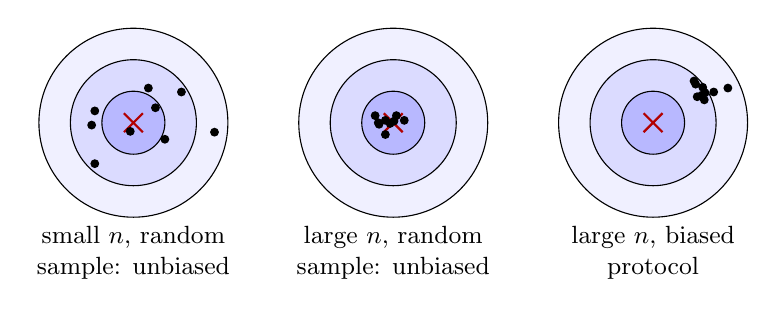
\begin{tikzpicture}
  \begin{scope}[xshift=0cm]
    \draw[fill=blue!6] (0,0) circle (1.2);
    \draw[fill=blue!14] (0,0) circle (0.8);
    \draw[fill=blue!28] (0,0) circle (0.4);
    \draw[red!70!black, thick] (-0.12,-0.12) -- (0.12,0.12) (-0.12,0.12) -- (0.12,-0.12);
    \fill[black] (-0.49,0.15) circle (1.6pt);
    \fill[black] (0.40,-0.21) circle (1.6pt);
    \fill[black] (-0.53,-0.03) circle (1.6pt);
    \fill[black] (0.19,0.44) circle (1.6pt);
    \fill[black] (-0.49,-0.52) circle (1.6pt);
    \fill[black] (0.28,0.19) circle (1.6pt);
    \fill[black] (0.61,0.39) circle (1.6pt);
    \fill[black] (-0.04,-0.11) circle (1.6pt);
    \fill[black] (1.03,-0.12) circle (1.6pt);
    \node[font=\small, align=center] at (0,-1.65) {small $n$, random\\sample: unbiased};
  \end{scope}
  \begin{scope}[xshift=3.3cm]
    \draw[fill=blue!6] (0,0) circle (1.2);
    \draw[fill=blue!14] (0,0) circle (0.8);
    \draw[fill=blue!28] (0,0) circle (0.4);
    \draw[red!70!black, thick] (-0.12,-0.12) -- (0.12,0.12) (-0.12,0.12) -- (0.12,-0.12);
    \fill[black] (-0.10,-0.15) circle (1.6pt);
    \fill[black] (0.01,0.02) circle (1.6pt);
    \fill[black] (-0.04,-0.01) circle (1.6pt);
    \fill[black] (0.04,0.09) circle (1.6pt);
    \fill[black] (0.14,0.03) circle (1.6pt);
    \fill[black] (-0.23,0.09) circle (1.6pt);
    \fill[black] (-0.18,-0.02) circle (1.6pt);
    \fill[black] (-0.19,0.00) circle (1.6pt);
    \fill[black] (-0.10,0.03) circle (1.6pt);
    \node[font=\small, align=center] at (0,-1.65) {large $n$, random\\sample: unbiased};
  \end{scope}
  \begin{scope}[xshift=6.6cm]
    \draw[fill=blue!6] (0,0) circle (1.2);
    \draw[fill=blue!14] (0,0) circle (0.8);
    \draw[fill=blue!28] (0,0) circle (0.4);
    \draw[red!70!black, thick] (-0.12,-0.12) -- (0.12,0.12) (-0.12,0.12) -- (0.12,-0.12);
    \fill[black] (0.95,0.44) circle (1.6pt);
    \fill[black] (0.65,0.29) circle (1.6pt);
    \fill[black] (0.52,0.53) circle (1.6pt);
    \fill[black] (0.54,0.49) circle (1.6pt);
    \fill[black] (0.56,0.33) circle (1.6pt);
    \fill[black] (0.62,0.35) circle (1.6pt);
    \fill[black] (0.77,0.39) circle (1.6pt);
    \fill[black] (0.63,0.45) circle (1.6pt);
    \fill[black] (0.66,0.38) circle (1.6pt);
    \node[font=\small, align=center] at (0,-1.65) {large $n$, biased\\protocol};
  \end{scope}
\end{tikzpicture}
\end{center}
The cross marks the attribute of interest and each dot is the estimate from one possible
sample. A bigger sample pulls the dots together (less sample error) but cannot move their
centre: a biased protocol stays biased however large $n$ is.

\section*{Summary}
\begin{itemize}
  \item PPDAC: Problem (population, variates, attributes, question), Plan (study
        population, sampling protocol, measurement), Data, Analysis, Conclusion.
  \item Study error (target vs study population), sample error (sample vs study
        population; quantifiable under random sampling), measurement error (measured vs
        true value).
  \item Simple random sampling is the basic protocol justifying probability models;
        stratified, cluster and systematic sampling are variations; convenience samples
        are unreliable.
\end{itemize}
